\section{Robot Hand Base}

\subsection{Middle Plate}

\begin{table}[ht!]
  	\begin{minipage}[b]{0.50\linewidth}\centering
	\scalebox{0.97}{
	\begin{tabular}{ | c | c |}
		\hline
		{\bf{Part}} & {\bf{Qty}}\\ \hline
    		MiddlePlate & 1  \\ \hline
    		M3Spacer30 & 8  \\ \hline
		M3ThreadedRod & 4 \\ \hline
    	\end{tabular}
	}
	\end{minipage}
	\hspace{0.5cm}	
	\begin{minipage}[b]{0.50\linewidth}\centering
	\scalebox{1}{
	\begin{tabular}{ | c |}
		\hline
 		\multicolumn{1}{|c|}{{\bf{Tools}}} \\
		\hline
		Open-End Wrench \\ \hline
    	\end{tabular}
	}
  	\end{minipage}

\end{table}

\vspace{0.5cm}

\begin{center}
\begin{tikzpicture}
\node [mybox] (box){%
  	\begin{minipage}[b]{0.50\linewidth}\centering
	\begin{tabular}{ c }
		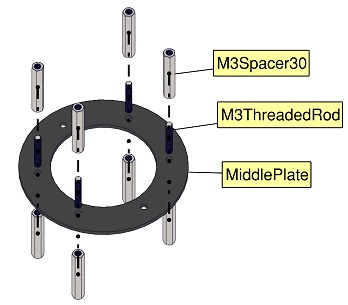
\includegraphics[width = 6cm]{figures/Base/Base1.jpg}
    	\end{tabular}
	\end{minipage}
	\hspace{0.5cm}	
	\begin{minipage}[b]{0.50\linewidth}
	\begin{tabular}{ l }
		\Circled{1} Tighten the M3ThreadedRod until \\ the midway (12mm). \\
		\Circled{2} Continue as you see in the picture.
    	\end{tabular}
  	\end{minipage}
};
\node[mytitle, right=10pt] at (box.north west) {7.1.1};
\end{tikzpicture}%
\end{center}

\subsection{Bearing Base}

\begin{table}[ht!]
  	\begin{minipage}[b]{0.50\linewidth}\centering
	\scalebox{0.97}{
	\begin{tabular}{ | c | c |}
		\hline
		{\bf{Part}} & {\bf{Qty}}\\ \hline
    		BearingBase & 4  \\ \hline
		pulley & 1 \\ \hline
		M3x20 & 1 \\ \hline
		M3Washer & 3 \\ \hline
		PlasticSpacer & 2 \\ \hline
		M3Nut & 1 \\ \hline
    	\end{tabular}
	}
	\end{minipage}
	\hspace{0.5cm}	
	\begin{minipage}[b]{0.50\linewidth}\centering
	\scalebox{1}{
	\begin{tabular}{ | c |}
		\hline
 		\multicolumn{1}{|c|}{{\bf{Tools}}} \\
		\hline
		Open-End Wrench \\ \hline
		Acrylic Glue \\ \hline
		Allen Wrench \\ \hline
    	\end{tabular}
	}
  	\end{minipage}
\end{table}

\begin{center}
\begin{tikzpicture}
\node [mybox] (box){%
  	\begin{minipage}[b]{0.50\linewidth}\centering
	\begin{tabular}{ c }
           	     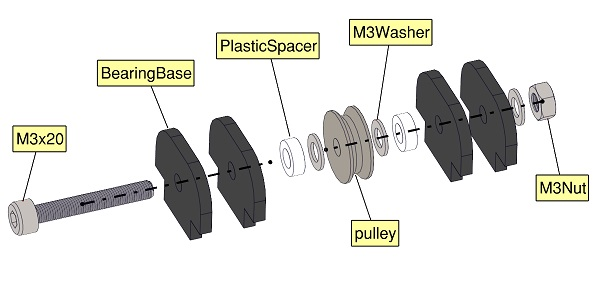
\includegraphics[width = 8cm]{figures/Base/Base2.jpg} 
    	\end{tabular}
	\end{minipage}
	\hspace{0.5cm}	
	\begin{minipage}[b]{0.50\linewidth}
	\begin{tabular}{ l }
		\Circled{1} Center the two BearingBase parts. \\
		\Circled{2} Glue the two BearingBase parts. \\
		\Circled{3} Repeat the same steps for the \\ second BearingBase. \\
    	\end{tabular}
  	\end{minipage}
};
\node[mytitle, right=10pt] at (box.north west) {7.2.1};
\end{tikzpicture}%
\end{center}

\newpage

\subsection{Bottom Plate with AX12 Servo}

\begin{table}[ht!]
  	\begin{minipage}[b]{0.50\linewidth}\centering
	\scalebox{0.97}{
	\begin{tabular}{ | c | c |}
		\hline
		{\bf{Part}} & {\bf{Qty}}\\ \hline
    		BearingBase & 4  \\ \hline
    		BottomPlateAX12 & 2  \\ \hline
                PCBMount & 1 \\ \hline
		AX12Base & 1 \\ \hline
		M2x8 & 4 \\ \hline
		M2Nut & 4 \\ \hline
    	\end{tabular}
	}
	\end{minipage}
	\hspace{0.5cm}	
	\begin{minipage}[b]{0.50\linewidth}\centering
	\scalebox{1}{
	\begin{tabular}{ | c |}
		\hline
 		\multicolumn{1}{|c|}{{\bf{Tools}}} \\
		\hline
		Open-End Wrench \\ \hline
		Acrylic Glue \\ \hline
		Allen Wrench \\ \hline
    	\end{tabular}
	}
  	\end{minipage}
\end{table}

\begin{center}
\begin{tikzpicture}
\node [mybox] (box){%
  	\begin{minipage}[b]{0.50\linewidth}\centering
	\begin{tabular}{ l }
		\Circled{1} Center the two BottomPlate parts. \\
		\Circled{2} Glue the two BottomPlate parts. \\
		\Circled{3} Glue the BearingBase to the \\ BottomPlateAX12 with acrylic glue. \\
                \Circled{4} Glue the PCBMount to the BottomPlateAX12. \\
    	\end{tabular}
	\end{minipage}
	\hspace{0.5cm}	
	\begin{minipage}[b]{0.50\linewidth}
	\begin{tabular}{ l }
 	 	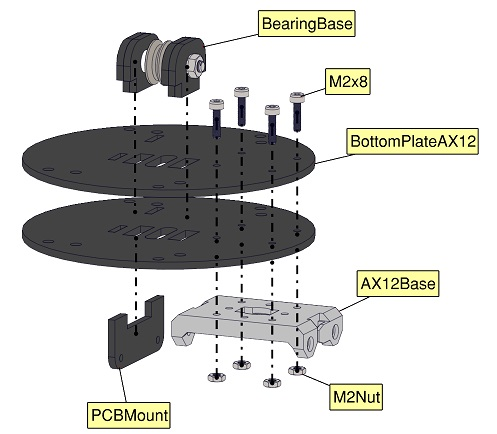
\includegraphics[width = 7cm]{figures/Base/Base3.jpg} 
    	\end{tabular}
  	\end{minipage}
};
\node[mytitle, right=10pt] at (box.north west) {7.3.1};
\end{tikzpicture}%
\end{center}

\newpage

\subsection{Bottom Plate with Standard Servo}

\begin{table}[ht!]
  	\begin{minipage}[b]{0.50\linewidth}\centering
	\scalebox{0.97}{
	\begin{tabular}{ | c | c |}
		\hline
		{\bf{Part}} & {\bf{Qty}}\\ \hline
    		BottomPlateStdServo & 2  \\ \hline
    		BearingBase & 1  \\ \hline
		stdServoBase & 6 \\ \hline
                PCBMount & 1 \\ \hline
		M3x12 & 2 \\ \hline
		M3Washer & 2 \\ \hline
		M3Nut & 2 \\ \hline
    	\end{tabular}
	}
	\end{minipage}
	\hspace{0.5cm}	
	\begin{minipage}[b]{0.50\linewidth}\centering
	\scalebox{1}{
	\begin{tabular}{ | c |}
		\hline
 		\multicolumn{1}{|c|}{{\bf{Tools}}} \\
		\hline
		Allen Wrench \\ \hline
		Acrylic Glue \\ \hline
    	\end{tabular}
	}
  	\end{minipage}
\end{table}

\vspace{0.2cm}

\begin{center}
\begin{tikzpicture}
\node [mybox] (box){%
  	\begin{minipage}[b]{0.50\linewidth}\centering
	\begin{tabular}{ c }
		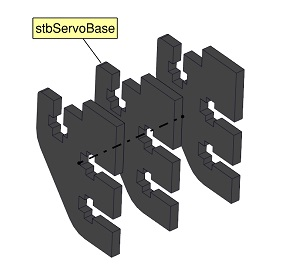
\includegraphics[width = 4cm]{figures/Base/Base4.jpg}
    	\end{tabular}
	\end{minipage}
	\hspace{0.5cm}	
	\begin{minipage}[b]{0.50\linewidth}
	\begin{tabular}{ l }
		\Circled{1} Center the two stdServoBase parts. \\
		\Circled{2} Glue the two stdServoBase parts. \\
		\Circled{3} Center the third stdServoBase part\\ with the other two. \\
		\Circled{4} Glue the third stdServoBase part\\ with the other two. \\
    	\end{tabular}
  	\end{minipage}
};
\node[mytitle, right=10pt] at (box.north west) {7.4.1};
\end{tikzpicture}%
\end{center}

\vspace{0.2cm}

\begin{center}
\begin{tikzpicture}
\node [mybox] (box){%
  	\begin{minipage}[b]{0.50\linewidth}\centering
	\begin{tabular}{ l }
		\Circled{1} Center the BottomPlateStdServo \\ as you see in the picture. \\
		\Circled{2} Glue the two parts with acrylic glue. \\
		\Circled{3} Center the BearingBase with the \\ BottomPlateStdServo as you see in the picture. \\
		\Circled{4} Glue the two parts with acrylic glue. \\
                \Circled{5} Glue the PCBMount to the\\ BottomPlateStdServo. \\
		\Circled{6} Continue as you see in the picture.
    	\end{tabular}
	\end{minipage}
	\hspace{0.5cm}	
	\begin{minipage}[b]{0.50\linewidth}
	\begin{tabular}{ c }
		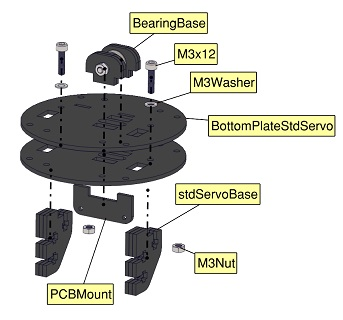
\includegraphics[width = 7cm]{figures/Base/Base5.jpg}
    	\end{tabular}
  	\end{minipage}
};
\node[mytitle, right=10pt] at (box.north west) {7.4.2};
\end{tikzpicture}%
\end{center}

\newpage

\subsection{Robot Base with AX12 Servo}

\begin{table}[ht!]
  	\begin{minipage}[b]{0.50\linewidth}\centering
	\scalebox{0.97}{
	\begin{tabular}{ | c | c |}
		\hline
		{\bf{Part}} & {\bf{Qty}}\\ \hline
		MiddlePlate& 1 \\ \hline
		BottomPlateAX12 & 1 \\ \hline
		FingersTopPlate & 1 \\ \hline
		M3x10 & 8 \\ \hline
		M3Washer & 8 \\ \hline
    	\end{tabular}
	}
	\end{minipage}
	\hspace{0.5cm}	
	\begin{minipage}[b]{0.50\linewidth}\centering
	\scalebox{1}{
	\begin{tabular}{ | c |}
		\hline
 		\multicolumn{1}{|c|}{{\bf{Tools}}} \\
		\hline
		Open-End Wrench \\ \hline
		Allen Wrench\\ \hline
    	\end{tabular}
	}
  	\end{minipage}
\end{table}

\vspace{0.5cm}

\begin{center}
\begin{tikzpicture}
\node [mybox] (box){%
	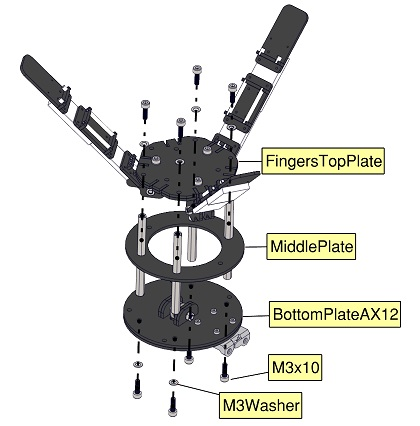
\includegraphics[width = 9cm]{figures/Base/Base6.jpg}
};
\node[mytitle, right=10pt] at (box.north west) {7.5.1};
\end{tikzpicture}%
\end{center}

\newpage

\subsection{Robot Base with Standard Servo}

\begin{table}[ht!]
  	\begin{minipage}[b]{0.50\linewidth}\centering
	\scalebox{0.97}{
	\begin{tabular}{ | c | c |}
		\hline
		{\bf{Part}} & {\bf{Qty}}\\ \hline
		MiddlePlate & 1 \\ \hline
		BottomPlateStdServo & 1 \\ \hline
		FingersTopPlate& 1 \\ \hline
		M3x10 & 8 \\ \hline
		M3Washer & 8 \\ \hline
    	\end{tabular}
	}
	\end{minipage}
	\hspace{0.5cm}	
	\begin{minipage}[b]{0.50\linewidth}\centering
	\scalebox{1}{
	\begin{tabular}{ | c |}
		\hline
 		\multicolumn{1}{|c|}{{\bf{Tools}}} \\
		\hline
		Open-End Wrench \\ \hline
		Allen Wrench\\ \hline
    	\end{tabular}
	}
  	\end{minipage}
\end{table}

\vspace{0.5cm}

\begin{center}
\begin{tikzpicture}
\node [mybox] (box){%
	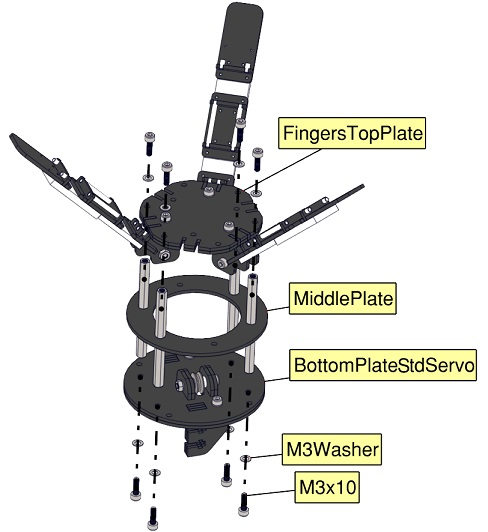
\includegraphics[width = 9cm]{figures/Base/Base7.jpg}
};
\node[mytitle, right=10pt] at (box.north west) {7.6.1};
\end{tikzpicture}%
\end{center}

\newpage

\subsection{AX12 Servo}

\begin{table}[ht!]
  	\begin{minipage}[b]{0.50\linewidth}\centering
	\scalebox{0.97}{
	\begin{tabular}{ | c | c |}
		\hline
		{\bf{Part}} & {\bf{Qty}}\\ \hline
		AX12Base & 1\\ \hline
		servoPulleyAX12 \#1 & 1 \\ \hline
		servoPulleyAX12 \#2 & 1 \\ \hline
		servoPulleyAX12 \#3 & 1 \\ \hline
		AX12 Servo& 1 \\ \hline
		M2x8 & 4 \\ \hline
		M2Nut & 4 \\ \hline
		M2x6 & 2 \\ \hline
		M2.5x15 & 1  \\ \hline
    	\end{tabular}
	}
	\end{minipage}
	\hspace{0.5cm}	
	\begin{minipage}[b]{0.50\linewidth}\centering
	\scalebox{1}{
	\begin{tabular}{ | c |}
		\hline
 		\multicolumn{1}{|c|}{{\bf{Tools}}} \\
		\hline
		Acrylic Glue \\ \hline
		Allen Wrench\\ \hline
    	\end{tabular}
	}
  	\end{minipage}
\end{table}

\vspace{0.2cm}

\begin{center}
\begin{tikzpicture}
\node [mybox] (box){%
  	\begin{minipage}[b]{0.50\linewidth}\centering
	\begin{tabular}{ c }
		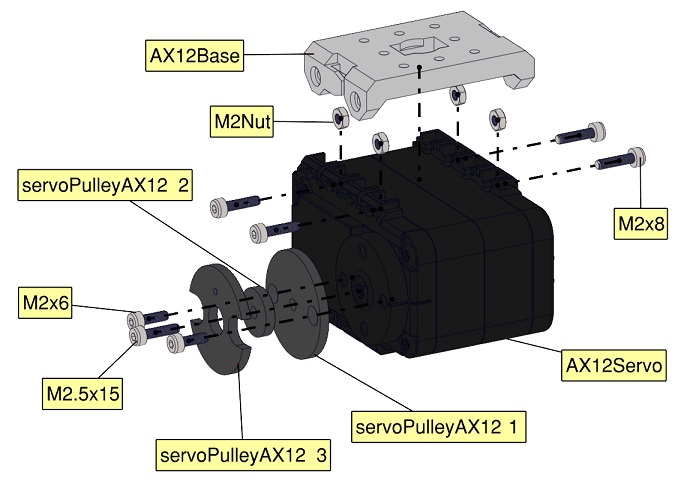
\includegraphics[width = 8cm]{figures/Base/Base12.jpg}
    	\end{tabular}
	\end{minipage}
	\hspace{0.5cm}	
	\begin{minipage}[b]{0.50\linewidth}
	\begin{tabular}{ l }
		\Circled{1} Center the servoPulleyAX12 parts \#1,2.\\
		\Circled{2} Glue the two parts with acrylic glue. \\
		\Circled{3} Center the servoPulleyAX12 parts \#1-2,3. \\
		\Circled{4} Glue the two parts with acrylic glue. \\
		\Circled{!} Press all the parts together\\ to achieve better gluing. \\
    	\end{tabular}
  	\end{minipage}
};
\node[mytitle, right=10pt] at (box.north west) {7.7.1};
\end{tikzpicture}%
\end{center}

\vspace{0.2cm}

\begin{center}
\begin{tikzpicture}
\node [mybox] (box){%
  	\begin{minipage}[b]{0.50\linewidth}\centering
	\begin{tabular}{ l }
		\Circled{1} Insert a Dyneema edge in the anchor hole. \\
		\Circled{2} With the edge of the Dyneema and the M3Nut \\ do multiple surgeon's knots. \\
		\Circled{3} Wrap the dyneema around the servo pulley \\ until taut. \\
		\Circled{!} You can adjust the initial configuration later\\ zeroing the servo motor.\\ 
		\Circled{4} Screw the M2.5x15 to the AX12 servo.
    	\end{tabular}
	\end{minipage}
	\hspace{0.5cm}	
	\begin{minipage}[b]{0.50\linewidth}
	\begin{tabular}{ c }
		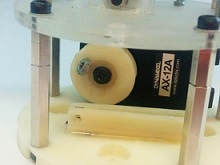
\includegraphics[width = 7cm]{figures/Base/Base14.jpg}
    	\end{tabular}
  	\end{minipage}
};
\node[mytitle, right=10pt] at (box.north west) {7.7.2 };
\end{tikzpicture}%
\end{center}

\newpage

\subsection{Standard Servo}

\begin{table}[ht!]
  	\begin{minipage}[b]{0.50\linewidth}\centering
	\scalebox{0.97}{
	\begin{tabular}{ | c | c |}
		\hline
		{\bf{Part}} & {\bf{Qty}}\\ \hline
		Robot Base StdServo & 1 \\ \hline
		servoPulleyStd1 & 1 \\ \hline
		servoPulleyStd2 & 1 \\ \hline
		servoPulleyStd3 & 1 \\ \hline
		Hitec HS-311 & 1 \\ \hline
		servoScrew & 1 \\ \hline
		M3x12 & 4 \\ \hline
		M3Washer & 4 \\ \hline
		M3Nut & 4 \\ \hline
    	\end{tabular}
	}
	\end{minipage}
	\hspace{0.5cm}	
	\begin{minipage}[b]{0.50\linewidth}\centering
	\scalebox{1}{
	\begin{tabular}{ | c |}
		\hline
 		\multicolumn{1}{|c|}{{\bf{Tools}}} \\
		\hline
		Acrylic Glue \\ \hline
		Allen Wrench\\ \hline
    	\end{tabular}
	}
  	\end{minipage}
\end{table}

\vspace{0.2cm}

\begin{center}
\begin{tikzpicture}
\node [mybox] (box){%
  	\begin{minipage}[b]{0.50\linewidth}\centering
	\begin{tabular}{ c }
		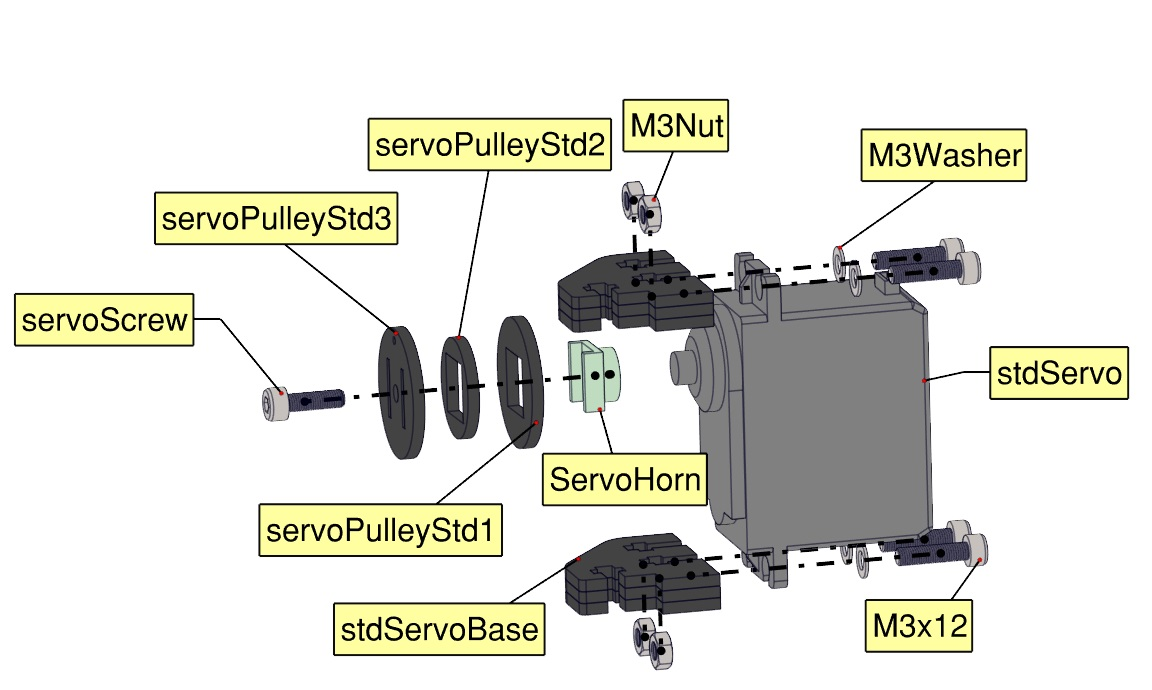
\includegraphics[width = 8cm]{figures/Base/Base13.jpg}
    	\end{tabular}
	\end{minipage}
	\hspace{0.5cm}	
	\begin{minipage}[b]{0.50\linewidth}
	\begin{tabular}{ l }
		\Circled{1} Center the servoPulleyStd parts \#1,2.\\
		\Circled{2} Glue the two parts with acrylic glue.\\
		\Circled{3} Center the servoPulleyStd parts \#1-2,3.\\
		\Circled{4} Glue the two parts with acrylic glue.\\
		\Circled{!} Press all parts together to achieve\\ better gluing. \\ 
		\Circled{5} Insert the edge of the Dyneema inside\\ the anchor hole of the servoPulleyStd part \#3.\\
		\Circled{6} With the edge of the Dyneema and the M3Nut \\ do multiple surgeon's knots. \\
		\Circled{7} Wrap the dyneema around the servo pulley \\ until taut. \\
		\Circled{!} You can adjust the initial configuration later\\ zeroing the servo motor.\\ 
		\Circled{8} Screw the servoScrew to the Hitec HS-311. \\
    	\end{tabular}
  	\end{minipage}
};
\node[mytitle, right=10pt] at (box.north west) {7.8.1};
\end{tikzpicture}%
\end{center}

\newpage

\subsection{Robot Flange for Robot Base with AX12 Servo}

\begin{table}[ht!]
  	\begin{minipage}[b]{0.50\linewidth}\centering
	\scalebox{0.97}{
	\begin{tabular}{ | c | c |}
		\hline
		{\bf{Part}} & {\bf{Qty}}\\ \hline
		flangeAX12 \#1 & 1 \\ \hline
		flangeAX12 \#2 & 1 \\ \hline
		flangeAX12 \#3 & 1 \\ \hline
		M3Spacer10 & 4 \\ \hline
		M3Spacer25 & 4 \\ \hline
		M3x10 & 4 \\ \hline
    	\end{tabular}
	}
	\end{minipage}
	\hspace{0.5cm}	
	\begin{minipage}[b]{0.50\linewidth}\centering
	\scalebox{1}{
	\begin{tabular}{ | c |}
		\hline
 		\multicolumn{1}{|c|}{{\bf{Tools}}} \\
		\hline
		Acrylic Glue \\ \hline
		Allen Wrench\\ \hline
		Open-End Wrench \\ \hline
    	\end{tabular}
	}
  	\end{minipage}
\end{table}

\vspace{0.5cm}

\begin{center}
\begin{tikzpicture}
\node [mybox] (box){%
  	\begin{minipage}[b]{0.50\linewidth}\centering
	\begin{tabular}{ c }
		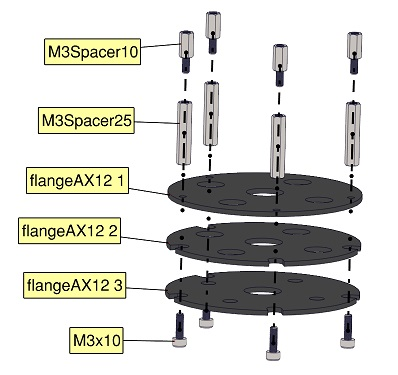
\includegraphics[width = 8cm]{figures/Base/Base8.jpg}
    	\end{tabular}
	\end{minipage}
	\hspace{0.5cm}	
	\begin{minipage}[b]{0.50\linewidth}
	\begin{tabular}{ l }
		\Circled{1} Center the flangeAX12 parts \#2,3.\\
		\Circled{2} Glue the two parts with acrylic glue.\\
		\Circled{3} Center the flangeAX12 parts \#1,2-3.\\
		\Circled{4} Glue the two parts with acrylic glue. \\
    	\end{tabular}
  	\end{minipage}
};
\node[mytitle, right=10pt] at (box.north west) {7.9.1};
\end{tikzpicture}%
\end{center}

\newpage

\subsection{Robot Flange for Robot Base with Standard Servo}

\begin{table}[ht!]
  	\begin{minipage}[b]{0.50\linewidth}\centering
	\scalebox{0.97}{
	\begin{tabular}{ | c | c |}
		\hline
		{\bf{Part}} & {\bf{Qty}}\\ \hline
		flangeStdServo \#1 & 1 \\ \hline
		flangeStdServo \#2 & 1 \\ \hline
		flangeStdServo \#3 & 1 \\ \hline
		M3Spacer10 & 4 \\ \hline
		M3Spacer25 & 4 \\ \hline
		M3x10 & 4 \\ \hline
    	\end{tabular}
	}
	\end{minipage}
	\hspace{0.5cm}	
	\begin{minipage}[b]{0.50\linewidth}\centering
	\scalebox{1}{
	\begin{tabular}{ | c |}
		\hline
 		\multicolumn{1}{|c|}{{\bf{Tools}}} \\
		\hline
		Acrylic Glue \\ \hline
		Allen Wrench\\ \hline
		Open-End Wrench \\ \hline
    	\end{tabular}
	}
  	\end{minipage}
\end{table}

\vspace{0.5cm}

\begin{center}
\begin{tikzpicture}
\node [mybox] (box){%
  	\begin{minipage}[b]{0.50\linewidth}\centering
	\begin{tabular}{ c }
		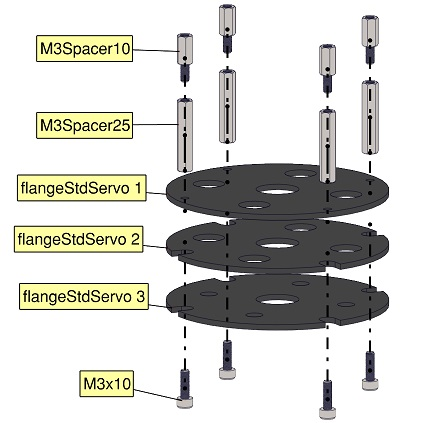
\includegraphics[width = 8cm]{figures/Base/Base9.jpg}
    	\end{tabular}
	\end{minipage}
	\hspace{0.5cm}	
	\begin{minipage}[b]{0.50\linewidth}
	\begin{tabular}{ l }
		\Circled{1} Center the flangeStdServo parts \#1,2.\\
		\Circled{2} Glue the two parts with acrylic glue. \\
		\Circled{3} Center the flangeStdServo parts \#1-2,3. \\
		\Circled{4} Glue the parts with acrylic glue. \\
		\Circled{5} Continue as you see in the picture.
    	\end{tabular}
  	\end{minipage}
};
\node[mytitle, right=10pt] at (box.north west) {7.10.1};
\end{tikzpicture}%
\end{center}

\newpage

\subsection{Final Assembly of Robot Hand with AX12 Servo}

\begin{table}[ht!]
  	\begin{minipage}[b]{0.50\linewidth}\centering
	\scalebox{0.97}{
	\begin{tabular}{ | c | c |}
		\hline
		{\bf{Part}} & {\bf{Qty}}\\ \hline
		FlangeAX12  & 1 \\ \hline
		Robot Hand AX12 & 1 \\ \hline
		M3Washer & 4 \\ \hline
		M3x10 & 4 \\ \hline
    	\end{tabular}
	}
	\end{minipage}
	\hspace{0.5cm}	
	\begin{minipage}[b]{0.50\linewidth}\centering
	\scalebox{1}{
	\begin{tabular}{ | c |}
		\hline
 		\multicolumn{1}{|c|}{{\bf{Tools}}} \\
		\hline
		Allen Wrench\\ \hline
		Open-End Wrench \\ \hline
    	\end{tabular}
	}
  	\end{minipage}
\end{table}

\vspace{0.5cm}

\begin{center}
\begin{tikzpicture}
\node [mybox] (box){%
	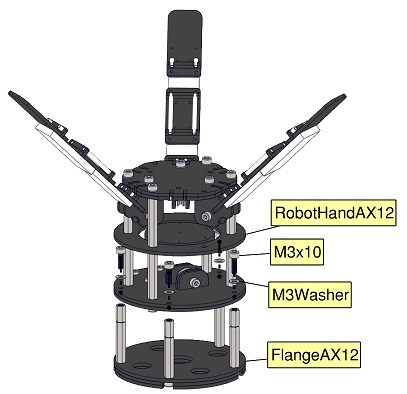
\includegraphics[width = 9cm]{figures/Base/Base11.jpg}
};
\node[mytitle, right=10pt] at (box.north west) {7.11.1};
\end{tikzpicture}%
\end{center}

\newpage

\subsection{Final Assembly of Robot Hand with Standard Servo}

\begin{table}[ht!]
  	\begin{minipage}[b]{0.50\linewidth}\centering
	\scalebox{0.97}{
	\begin{tabular}{ | c | c |}
		\hline
		{\bf{Part}} & {\bf{Qty}}\\ \hline
		FlangeStdServo & 1 \\ \hline
		Robot Hand stdServo & 1 \\ \hline
		M3Washer & 4 \\ \hline
		M3x10 & 4 \\ \hline
    	\end{tabular}
	}
	\end{minipage}
	\hspace{0.5cm}	
	\begin{minipage}[b]{0.50\linewidth}\centering
	\scalebox{1}{
	\begin{tabular}{ | c |}
		\hline
 		\multicolumn{1}{|c|}{{\bf{Tools}}} \\
		\hline
		Allen Wrench\\ \hline
		Open-End Wrench \\ \hline
    	\end{tabular}
	}
  	\end{minipage}
\end{table}

\vspace{0.5cm}

\begin{center}
\begin{tikzpicture}
\node [mybox] (box){%
	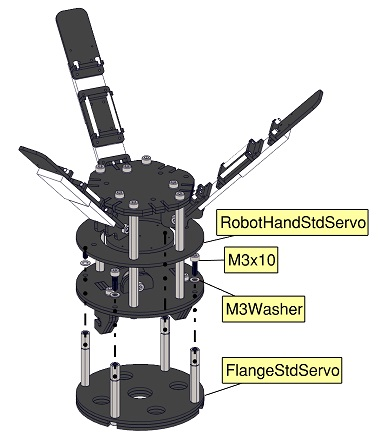
\includegraphics[width = 9cm]{figures/Base/Base10.jpg}
};
\node[mytitle, right=10pt] at (box.north west) {7.12.1};
\end{tikzpicture}%
\end{center}

\vspace{2cm}
\begin{center}
{\Large Congratulations you have created a robot hand!!!}
\end{center}
